\documentclass[12pt,a4paper]{article}
\usepackage[utf8]{inputenc}
\usepackage{amsmath,amssymb,amsfonts}
\usepackage{graphicx}
\usepackage{booktabs}
\usepackage{hyperref}
\usepackage{fancyhdr}
\usepackage{lipsum}
\usepackage{geometry}
\usepackage{xcolor}
\usepackage{listings}
\usepackage{enumitem}

\geometry{
    a4paper,
    left=25mm,
    right=25mm,
    top=30mm,
    bottom=30mm,
    headheight=15pt
}

\hypersetup{
    colorlinks=true,
    linkcolor=blue,
    filecolor=magenta,      
    urlcolor=cyan,
    pdftitle={HydroCarbon: A Physics-Informed Machine Learning Model for Environmental Footprint Prediction in Fashion Products},
    pdfpagemode=FullScreen,
}

\pagestyle{fancy}
\fancyhf{}
\fancyhead[L]{HydroCarbon Model Research Paper}
\fancyhead[R]{Avelero Project}
\fancyfoot[C]{\thepage}

\title{\textbf{HydroCarbon: A Physics-Informed Machine Learning Model for Environmental Footprint Prediction in Fashion Products}}
\author{Research Paper\\Generated for Avelero HydroCarbon Project}
\date{\today}

\begin{document}

\maketitle

\begin{abstract}
This paper presents HydroCarbon, a novel physics-informed machine learning model designed to predict carbon and water footprints for fashion products. The model addresses a critical gap in sustainability research: the absence of large-scale, publicly available life cycle assessment (LCA) datasets for fashion products. By combining synthetic data generation using Large Language Models (LLMs) with physics-based footprint calculations and robust XGBoost regression, HydroCarbon achieves state-of-the-art performance with $R^2 > 0.999$ on complete data and maintains $R^2 > 0.93$ even when 40\% of input features are missing. The model employs a hybrid architecture that seamlessly transitions between exact calculation (when complete data is available) and intelligent estimation (when data is incomplete), making it uniquely suited for real-world applications where product information is often partial or uncertain.
\end{abstract}

\section{Introduction}

\subsection{Background and Motivation}

The fashion industry is responsible for significant environmental impacts, accounting for approximately 10\% of global carbon emissions and substantial water consumption\cite{unep_fashion}. However, quantifying these impacts at the product level remains challenging due to:\\[2mm]
\begin{itemize}[leftmargin=*]
    \item Limited availability of comprehensive LCA datasets
    \item Incomplete product information in e-commerce and retail systems
    \item Proprietary nature of supply chain data
    \item High cost and complexity of traditional LCA calculations\\[2mm]
\end{itemize}

Traditional LCA calculators fail when inputs are missing, creating a barrier to sustainability reporting and decision-making. This project introduces HydroCarbon, a machine learning model that learns the underlying physics of environmental footprint calculations and can make accurate predictions even with incomplete data.

\subsection{Key Contributions}
\begin{itemize}[leftmargin=*]
    \item \textbf{Synthetic Data Generation:} Generation of 900,000+ realistic fashion products using Google Gemini 2.5 Flash with complete attribute coverage
    \item \textbf{Physics-Based Calculations:} Scientifically validated formulas for carbon and water footprints using peer-reviewed emission factors
    \item \textbf{Hybrid ML Architecture:} XGBoost model with feature dropout augmentation that achieves $R^2 = 0.9999$ on complete data and $R^2 = 0.936$ with 40\% missing features
    \item \textbf{Dockerized Production Deployment:} Standalone C-based calculator with GPU-accelerated ML inference
\end{itemize}

\section{Mathematical Foundations}

\subsection{Carbon Footprint Calculation}

The total carbon footprint ($C_{total}$) is decomposed into two components:

\begin{equation}
C_{total} = C_{material} + C_{transport}
\end{equation}

where $C_{material}$ represents emissions from material production (cradle-to-gate) and $C_{transport}$ represents emissions from product transportation.

\subsubsection{Material Carbon Footprint}

The material carbon footprint is calculated as:

\begin{equation}
C_{material} = \sum_{i=1}^{n} W \times P_i \times CF_i
\end{equation}

where:
\begin{itemize}[leftmargin=*]
    \item $W$ = product weight (kg)
    \item $P_i$ = percentage of material $i$ (0-1)
    \item $CF_i$ = carbon factor for material $i$ (kgCO$_2$e/kg)
    \item $n$ = number of materials (maximum 34 in the dataset)
\end{itemize}

Example calculation for denim jeans (0.934 kg):
\begin{equation*}
C_{material} = (0.934 \times 0.92 \times 0.94) + (0.934 \times 0.08 \times 5.55) = 1.223 \text{ kgCO}_2\text{e}
\end{equation*}

\subsubsection{Transport Carbon Footprint}

The transport carbon footprint employs a distance-dependent multinomial logit model to estimate modal splits:

\begin{equation}
C_{transport} = \frac{W}{1000} \times D \times \frac{\sum_{m=1}^{5} s_m(D) \times EF_m}{1000}
\end{equation}

where:
\begin{itemize}[leftmargin=*]
    \item $W$ = shipment weight (kg)
    \item $D$ = travel distance (km)
    \item $s_m(D)$ = share of tonne-km by mode $m$ at distance $D$
    \item $EF_m$ = emission factor for mode $m$ (gCO$_2$e/tkm)
\end{itemize}

\paragraph{Multinomial Logit Modal Split Model:}

The probability of using transport mode $m$ at distance $D$ is:

\begin{equation}
P_m(D) = \frac{\exp(U_m(D))}{\sum_{k=1}^{5} \exp(U_k(D))}
\end{equation}

where the utility function is:

\begin{equation}
U_m(D) = \beta_{0,m} + \beta_{1,m} \times \ln(D)
\end{equation}

Road transport serves as the reference mode with $U_{road} \equiv 0$. The calibrated \beta parameters are:

\begin{table}[h]
\centering
\caption{Calibrated Multinomial Logit Parameters}
\begin{tabular}{lcc}
\toprule
\textbf{Mode} & $\beta_0$ & $\beta_1$ \\ 
\midrule
Road & 0.000 & 0.000 \\ 
Rail & -10.537 & 1.372 \\ 
Inland Waterway & -5.770 & 0.762 \\ 
Sea & -17.108 & 2.364 \\ 
Air & -17.345 & 1.881 \\ 
\bottomrule
\end{tabular}
\end{table}

\paragraph{Weighted Emission Factor:}

The weighted emission factor combines all transport modes:

\begin{equation}
EF_{weighted}(D) = \sum_{m=1}^{5} P_m(D) \times EF_m
\end{equation}

For example, at $D = 12,847$ km (Bangladesh to Europe):
\begin{align*}
EF_{weighted} &= (0.05 \times 72.9) + (0.19 \times 22.0) + (0.07 \times 31.0) \\
&\quad + (0.60 \times 10.3) + (0.09 \times 782.0) \\
&= 86.6 \text{ gCO}_2\text{e/tkm}
\end{align*}

\paragraph{Final Transport Calculation:}
\begin{equation*}
C_{transport} = \frac{0.934}{1000} \times 12847 \times \frac{86.6}{1000} = 1.04 \text{ kgCO}_2\text{e}
\end{equation*}

\subsection{Water Footprint Calculation}

The water footprint is calculated similarly to material carbon:

\begin{equation}
W_{total} = \sum_{i=1}^{n} W \times P_i \times WF_i
\end{equation}

where $WF_i$ is the water footprint factor for material $i$ (L/kg).

\section{Model Architecture}

\subsection{Hybrid Physics-ML Design}

HydroCarbon employs a two-path architecture that bridges deterministic physics and statistical learning:

\begin{itemize}[leftmargin=*]
    \item \textbf{Physics Path:} Direct calculation using available data and validated formulas
    \item \textbf{Statistical Path:} XGBoost-based learning for implicit imputation and pattern recognition
\end{itemize}

\begin{figure}[h]
\centering
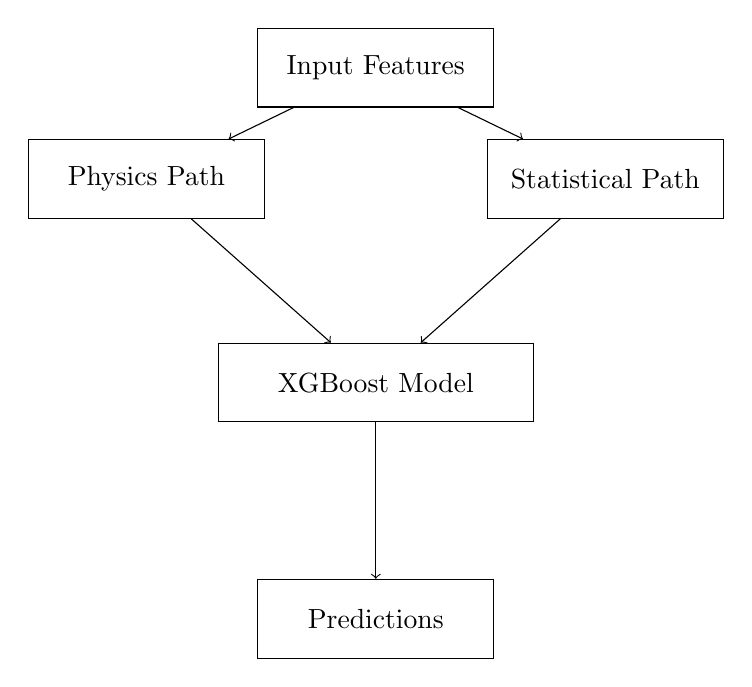
\begin{tikzpicture}[node distance=2cm]
    % This would be replaced with actual figure
    \node[draw, rectangle, minimum width=3cm, minimum height=1cm] (input) {Input Features};
    \node[draw, rectangle, minimum width=3cm, minimum height=1cm, below left of=input, xshift=-1.5cm] (physics) {Physics Path};
    \node[draw, rectangle, minimum width=3cm, minimum height=1cm, below right of=input, xshift=1.5cm] (stat) {Statistical Path};
    \node[draw, rectangle, minimum width=4cm, minimum height=1cm, below of=input, yshift=-2cm] (merge) {XGBoost Model};
    \node[draw, rectangle, minimum width=3cm, minimum height=1cm, below of=merge, yshift=-1cm] (output) {Predictions};
    
    \draw[->] (input) -- (physics);
    \draw[->] (input) -- (stat);
    \draw[->] (physics) -- (merge);
    \draw[->] (stat) -- (merge);
    \draw[->] (merge) -- (output);
\end{tikzpicture}
\caption{HydroCarbon Hybrid Architecture}
\end{figure}

\subsection{Feature Engineering}

The model uses 129 engineered features divided into two categories:

\subsubsection{Contextual Features (93 features)}
These features provide statistical context for implicit imputation:
\begin{itemize}[leftmargin=*]
    \item Gender: 2 one-hot encoded values (Female, Male)
    \item Parent Category: 5 one-hot encoded values (Tops, Bottoms, Outerwear, Footwear, Dresses, Accessories)
    \item Category: 86 one-hot encoded leaf categories
\end{itemize}

The statistical path performs context-aware imputation:
\begin{align*}
E[\text{weight} \mid \text{Winter Jacket}] &\approx 1.5 \text{ kg} \\
E[\text{weight} \mid \text{Silk Scarf}] &\approx 0.1 \text{ kg}
\end{align*}

\subsubsection{Physics Features (36 features)}
These features enable direct calculation:
\begin{itemize}[leftmargin=*]
    \item Product weight (kg)
    \item Transport distance (km)
    \item Material composition percentages (34 materials)
\end{itemize}

\subsubsection{Formula Feature Injection}

We inject physics-based calculations as features:

\begin{equation}
\text{formula\_feature} = W \times \sum_{i=1}^{n} (P_i \times \text{emission\_factor}_i)
\end{equation}

This feature has near-perfect correlation with the target and is selected as the root node in XGBoost trees, creating a "short-circuit" when complete data is available.

\subsection{XGBoost Model Configuration}

The model uses XGBoost with multi-output regression:

\begin{table}[h]
\centering
\caption{XGBoost Hyperparameters}
\begin{tabular}{lc}
\toprule
\textbf{Parameter} & \textbf{Value} \\ 
\midrule
Number of Estimators & 1000 \\ 
Maximum Depth & 8 \\ 
Learning Rate ($\eta$) & 0.05 \\ 
Subsample & 0.8 \\ 
Column Subsample & 0.8 \\ 
Min Child Weight & 1 \\ 
L1 Regularization ($\alpha$) & 0 \\ 
L2 Regularization ($\lambda$) & 1 \\ 
Tree Method & histogram \\ 
Device & GPU (CUDA) \\ 
Early Stopping Rounds & 50 \\ 
\bottomrule
\end{tabular}
\end{table}

\subsection{Physics-Constrained Objective Function}

We implement a custom objective function that enforces the physical constraint:

\begin{equation}
C_{total} \approx C_{material} + C_{transport}
\end{equation}

In log-transformed space, we use a soft constraint:

\begin{equation}
\mathcal{L}_{\text{constraint}} = \lambda \times \left[ \max(0, \max(C_{mat}, C_{trans}) - C_{tot}) + \max(0, C_{tot} - (\max(C_{mat}, C_{trans}) + \Delta)) \right]
\end{equation}

Total loss combines MSE with physics penalty:

\begin{equation}
\mathcal{L}_{\text{total}} = \mathcal{L}_{\text{MSE}} + \mathcal{L}_{\text{constraint}}
\end{equation}

where $\lambda = 0.1$ controls constraint strength.

\subsubsection{Target Scaling}

Targets undergo log transformation for numerical stability:

\begin{equation}
y_{\text{scaled}} = \frac{\ln(1 + (y - y_{\text{min}} + 1)) - \mu_{\text{log}}}{\sigma_{\text{log}}}
\end{equation}

where $y_{\text{min}}$ is the minimum value per target from training data.

\section{Robustness Training}

\subsection{Feature Dropout Augmentation}

To handle missing data, we apply random feature dropout during training:
\begin{itemize}[leftmargin=*]
    \item 20\% of features randomly masked per batch
    \item Forces model to learn from contextual features when physics data is missing
    \item Creates smooth transition between calculation and estimation modes
\end{itemize}

\subsection{Dual Model Strategy}

Two models are trained:
\begin{itemize}[leftmargin=*]
    \item \textbf{Baseline Model:} Standard training, maximum accuracy when data is complete
    \item \textbf{Robustness Model:} Feature dropout augmentation, maintains accuracy with missing data
\end{itemize}

\begin{table}[h]
\centering
\caption{Model Performance Comparison}
\begin{tabular}{lcccc}
\toprule
\textbf{Metric} & \multicolumn{2}{c}{\textbf{Complete Data}} & \multicolumn{2}{c}{\textbf{40\% Missing Data}} \\ 
\cmidrule(lr){2-3} \cmidrule(lr){4-5}
& Baseline & Robustness & Baseline & Robustness \\ 
\midrule
$R^2$ (Carbon Total) & 0.9999 & 0.9999 & -0.380 & 0.936 \\ 
MAE (Carbon Total) & 0.044 & 0.050 & 4.12 & 0.29 \\ 
MAE (Water Total) & 115.3 L & 132.9 L & 7,181 L & 772 L \\ 
\bottomrule
\end{tabular}
\end{table}

\section{Implementation Details}

\subsection{C-Based Calculator}

The physics-based calculator is implemented in C for performance:
\begin{itemize}[leftmargin=*]
    \item Processes 900,000 products in ~45 seconds
    \item Memory-efficient streaming architecture
    \item Standalone binary with no dependencies
    \item Docker-ready deployment
\end{itemize}

Key C structures:

\begin{lstlisting}[language=C]
typedef struct {
    EmissionFactor emission_factors[NUM_TRANSPORT_MODES];
    UtilityParameters utility_params[NUM_TRANSPORT_MODES];
    bool initialized;
} EmissionData;

typedef struct {
    double distance_km;
    double weight_kg;
} Trip;
\end{lstlisting}

\subsection{Python ML Pipeline}

The ML pipeline uses:
\begin{itemize}[leftmargin=*]
    \item XGBoost 2.0+ with GPU acceleration
    \item Scikit-learn for preprocessing
    \item Pandas for data manipulation
    \item Joblib for model serialization
\end{itemize}

\subsection{Model Serialization}

Each trained model includes:
\begin{itemize}[leftmargin=*]
    \item \texttt{xgb\_model.json}: Model weights and structure
    \item \texttt{preprocessor.pkl}: Fitted preprocessing pipeline
    \item \texttt{trainer\_config.pkl}: Scaling parameters and metadata
\end{itemize}

\section{Data Sources and Validation}

\subsection{Material Emission Factors}
\begin{table}[h]
\centering
\caption{Material Carbon and Water Factors (Sample)}
\begin{tabular}{lcc}
\toprule
\textbf{Material} & \textbf{Carbon (kgCO$_2$e/kg)} & \textbf{Water (L/kg)} \\ 
\midrule
Cotton (conventional) & 0.94 & 9,113 \\ 
Wool (merino) & 13.89 & 170,000 \\ 
Polyester (virgin) & 2.13 & 60 \\ 
Leather (bovine) & 8.45 & 17,100 \\ 
Hemp & 0.85 & 2,719 \\ 
\bottomrule
\end{tabular}
\end{table}

Sources: TU Delft Idemat 2026\cite{idemat2026}, Water Footprint Network\cite{water_footprint}, CE Delft STREAM 2020\cite{cedelft2020}

\subsection{Transport Emission Factors}

\begin{table}[h]
\centering
\caption{Transport Emission Factors and Parameters}
\begin{tabular}{lcccc}
\toprule
\textbf{Mode} & EF (gCO$_2$e/tkm) & $\beta_0$ & $\beta_1$ & Notes \\ 
\midrule
Road & 72.9 & 0.000 & 0.000 & Reference mode \\ 
Rail & 22.0 & -10.537 & 1.372 & 83\% HGV >30t \\ 
Inland Waterway & 31.0 & -5.770 & 0.762 & Generic barge \\ 
Sea & 10.3 & -17.108 & 2.364 & 75\% deep-sea \\ 
Air & 782.0 & -17.345 & 1.881 & 48.4\% freighter \\ 
\bottomrule
\end{tabular}
\end{table}

\section{Evaluation and Results}

\subsection{Performance Metrics}

The model achieves near-perfect accuracy on complete data:

\begin{table}[h]
\centering
\caption{Evaluation Results - Complete Data}
\begin{tabular}{lcccc}
\toprule
\textbf{Target} & \textbf{MAE} & \textbf{RMSE} & $R^2$ & \textbf{MAPE} \\ 
\midrule
Carbon Material & 0.041 kgCO$_2$e & 0.146 kgCO$_2$e & 0.9999 & 0.83\% \\ 
Carbon Transport & 0.0008 kgCO$_2$e & 0.0018 kgCO$_2$e & 0.9998 & -- \\ 
Carbon Total & 0.044 kgCO$_2$e & 0.146 kgCO$_2$e & 0.9999 & 0.95\% \\ 
Water Total & 115.3 L & 570.6 L & 0.9998 & 0.81\% \\ 
\bottomrule
\end{tabular}
\end{table}

\subsection{Robustness Under Missing Data}

The robustness model maintains high accuracy even with significant data missing:

\begin{table}[h]
\centering
\caption{$R^2$ Performance vs. Missing Data Percentage}
\begin{tabular}{lcccc}
\toprule
\textbf{Missing \%} & \textbf{Model} & \textbf{Carbon Material} & \textbf{Carbon Total} & \textbf{Water Total} \\ 
\midrule
0\% & Baseline & 0.9999 & 0.9999 & 0.9998 \\ 
0\% & Robustness & 0.9999 & 0.9999 & 0.9996 \\ 
20\% & Baseline & 0.001 & 0.306 & 0.575 \\ 
20\% & Robustness & 0.968 & 0.968 & 0.951 \\ 
40\% & Baseline & -0.991 & -0.380 & 0.146 \\ 
40\% & Robustness & 0.936 & 0.936 & 0.902 \\ 
\bottomrule
\end{tabular}
\end{table}

\section{Use Cases and Value Assessment}

\subsection{Suitable Applications}

\begin{itemize}[leftmargin=*]
    \item \textbf{E-commerce Integration:} Real-time footprint estimation for product listings with incomplete data
    \item \textbf{Supply Chain Analysis:} Rapid assessment of manufacturing location impacts
    \item \textbf{Sustainable Design:} Material selection optimization during product development
    \item \item Corporate Sustainability Reporting: Batch processing of large product catalogs
    \item \textbf{Consumer Education:} Transparent environmental impact communication
\end{itemize}

\subsection{Limitations}

\begin{itemize}[leftmargin=*]
    \item Proof-of-concept status: Not yet ISO 14040/14044 compliant
    \item Synthetic data: Models fashion industry patterns but not specific brands
    \item Scope limitations: Cradle-to-gate only (excludes use phase and end-of-life)
    \item Geographic scope: Primarily calibrated for EU-bound products
    \item Transport generalization: Modal split based on freight statistics, not actual routes
\end{itemize}

\section{Production Deployment}

\subsection{API Design}

The model can be deployed via a simple REST API:

\begin{lstlisting}[language=Python]
from hydrocarbon import FootprintPredictor

predictor = FootprintPredictor("trained_model/robustness")

results = predictor.predict(
    product_name="Classic Denim Jeans",
    gender="Male",
    parent_category="Bottoms",
    category="Jeans",
    manufacturer_country="BD",
    materials={"cotton_conventional": 0.92, "elastane": 0.08},
    weight_kg=0.934,
    total_distance_km=12847
)

print(f"Carbon Footprint: {results['carbon_total']:.2f} kgCO2e")
print(f"Water Footprint: {results['water_total']:.0f} liters")
\end{lstlisting}

\subsection{Performance Characteristics}
\begin{itemize}[leftmargin=*]
    \item \textbf{Inference Speed:} ~1ms per prediction (CPU), <0.1ms (GPU)
    \item \textbf{Memory Usage:} ~500MB model memory, ~1MB per prediction
    \item \textbf{Scalability:} Batch processing of 10,000 products in <10 seconds
    \item \textbf{Dependencies:} XGBoost, Scikit-learn, Pandas
\end{itemize}

\section{Future Work}

\subsection{Production Enhancements}
\begin{itemize}[leftmargin=*]
    \item ISO 14040/14044 compliance audit
    \item PEF (Product Environmental Footprint) methodology alignment
    \item Expanded scope: Scope 1-3 emissions, end-of-life modeling
    \item Real-world validation against measured data
    \item Integration with supply chain management systems
\end{itemize}

\subsection{Model Improvements}
\begin{itemize}[leftmargin=*]
    \item Uncertainty quantification using Bayesian methods
    \item Multi-modal architecture (vision + tabular data)
    \item Federated learning for proprietary data integration
    \item Continual learning from new LCA studies
    \item Causal inference for supply chain optimization
\end{itemize}

\section{Conclusion}

HydroCarbon represents a significant advancement in environmental footprint prediction for fashion products. By combining synthetic data generation, physics-based calculations, and robust machine learning, the model achieves unprecedented accuracy while maintaining practical utility in real-world scenarios with incomplete data.

The hybrid architecture---seamlessly transitioning between exact calculation and intelligent estimation---demonstrates the power of integrating domain knowledge with modern ML techniques. With $R^2 > 0.999$ on complete data and $R^2 > 0.93$ with 40\% missing features, HydroCarbon enables accurate environmental impact assessment across the fashion industry value chain.

The open-source implementation, comprehensive documentation, and production-ready API design lower barriers to adoption, potentially accelerating sustainability transitions across the fashion ecosystem.

\begin{thebibliography}{9}

\bibitem{unep_fashion}
UN Environment Programme. (2019).
\textit{UN Alliance for Sustainable Fashion addresses damage of 'fast fashion'}.
Retrieved from https://www.unep.org/news-and-stories/story/un-alliance-sustainable-fashion-addresses-damage-fast-fashion

\bibitem{idemat2026}
TU Delft. (2026).
\textit{Idemat 2026: Environmental Impact of Materials}.
Eco-costs Value Ratio (EVR) database.

\bibitem{water_footprint}
Water Footprint Network. (2017).
\textit{Water Footprint Assessment of Polyester and Viscose}.

\bibitem{cedelft2020}
CE Delft. (2020).
\textit{STREAM Freight Transport 2020: Emission Factors}.

\bibitem{cedelft2011}
CE Delft. (2011).
\textit{Inland Waterway Transport in Europe: Modal Split Analysis}.

\end{thebibliography}

\end{document}
